%! TeX program = lualatex
\documentclass{tp}
\usepackage{chemfig}
\usepackage{mhchem}
\usepackage{makecell}
\usepackage{pgfplots}
\titre{TP21 : Dosages acido-basiques}
\begin{document}
%\small


\section{Objectif du TP}
L'objectif de ce TP est de titrer une solution d'acide à l'aide d'un dosage acido-basique en utilisant trois méthodes différentes pour détecter l'équivalence : pH-métrie, conductimétrie et colorimétrie.

\section{Introduction}
Nous allons aborder ici trois méthodes de titrage acido-basique : pH-métrique, conductimétrique et colorimétrique. Le titrage pH-métrique permet d'obtenir le $\mathrm{pH}$ de la solution à tout instant, mais la détermination du point d'équivalence peut s'avérer délicate. La méthode conductimétrique permet d'obtenir le point d'équivalence avec précision dans tous les cas. La méthode colorimétrique est une méthode rapide et efficace à condition de choisir convenablement l'indicateur coloré et que le saut de $\mathrm{pH}$ soit suffisamment important.

L'exemple étudié ici est le titrage d'un acide faible, l'acide éthanoïque, par une solution d'hydroxyde de sodium (base forte), dont l'equation de réaction est

\begin{equation}
  \ce{CH3COOH(aq) + HO-(aq) -> CH3COO- (aq) + H2O(\ell)}
\end{equation}

La partie théorique présente l'intégralité des calculs permettant de prévoir la valeur de la quantité mesurée en chaque point de la courbe. Ils ne sont pas à connaitre in extenso, mais il n'est pas exclu de demander, pour un volume donné de réactif titrant versé, la composition du système et la valeur du pH ou de la conductivité.

\section{Partie théorique}%
\label{sec:partie_theorique}

\subsection{Définitions}%
\label{sub:definitions}

On appelle \textbf{dosage} toute technique destinée à déterminer une quantité de matière.

On appelle \textbf{titrage} un dosage qui fait intervenir une réaction chimique.

Une réaction chimique peut être utilisée comme réaction de titrage uniquement si elle est à la fois : totale, univoque (elle aboutit toujours aux mêmes produits) et rapide.

\subsection{Notations}%
\label{sub:notations}

On note: $V_a$, le volume d'acide versé dans le bécher, $c_a$ la concentration initiale de l'acide (qu'on cherche à déterminer), $V_b$ le volume de base versée, $V_\text{eq}$, le volume de base versé à l'équivalence et $c_b$ la concentration de la base dans la burette.
On introduira le paramètre sans dimension

\begin{equation}
  x=\frac{\text { quantité de réactif titrant ajouté }}{\text { quantité de réactif à titrer }}
\end{equation}
%
On a donc
\begin{equation}
  x = \frac{c_bV_b}{c_aV_a} \quad \text{or} \quad c_aV_a=c_bV_\text{eq} \quad \text{donc} \quad x=\frac{V_b}{V_\text{eq}}
\end{equation}

Il ne faut pas oublier de compter le volume de base versée dans le volume total, ni l'éventuel volume d'eau ajouté dans le bécher pour que les électrodes ou la cellule de conductimétrie trempent dans le mélange. Ces variations de volume ne modifient pas le volume équivalent (qui correspond à une égalité de quantités de matière), mais influent sur les concentrations et donc sur les grandeurs mesurées en cours de titrage (pH ou conductivité),

\subsection{Titrage pH-métrique}%
\label{sub:titrage_ph_metrique}

On remarquera que pour $x=1/2$ (point de demi-équivalence), $\pH=\pKa$. Autour de la demi-équivalence, le $\mathrm{pH}$ varie peu: on a une \textbf{solution tampon}, c'est-à-dire une solution dont le pH ne varie quasiment pas par ajout d'une faible quantité d'acide ou de base, ou par dilution.

Dans le tableau ci-dessous, on donne pour les différents instants du dosage les expression des concentrations des différentes espèces en solution et du pH en fonction de $x$. 

\begin{tabular}{llllll}
  \toprule
$x$ & $[\ce{CH3COOH}]$ & $[\ce{CH3COO-}]$  & $[\ce{H3O+}]$ & $[\ce{HO-}]$ & pH \\
  \midrule
  $x=0$ & $c_a$ & $\varepsilon_1$ & $\varepsilon_1$ & $\frac{K_e\cz^2}{\varepsilon_1}$  & $\frac{1}{2}\left( \pKa - \log\left( c_a/\cz \right)  \right) $  \\
  $x<1$ & $\frac{c_aV_a-c_bV_b}{V_a+V_b}$ & $\frac{c_bV_b}{V_a+V_b}$ & $\varepsilon_2$ & $\frac{K_e\cz^2}{\varepsilon_2}$ & $\pKa + \log\left( \frac{x}{1-x} \right) $ \\
  $x=1$ & $\varepsilon_3$ & $\frac{c_aV_a}{V_a+V_b} = \frac{c_bV_b}{V_a+V_b}$ & $\frac{K_e\cz^2}{\varepsilon_3}$ & $\varepsilon_3$ & $\frac{1}{2}\left( \pKa + \pKe + \log\left( \frac{c_b/\cz}{1+\frac{V_a}{V_\text{eq}}} \right)  \right) $ \\
  $x>1$ & $\varepsilon_4$ & $\frac{c_aV_a}{V_a+V_b} $ & $\frac{K_e\cz^2( V_a+V_b)}{c_bV_b-c_aV_a}$ & $\frac{c_bV_b-c_aV_a}{V_a+V_b}$ & $\pKe + \log\left( \frac{c_b}{\cz} \frac{x-1}{x+1} \right) $ \\
  \bottomrule
\end{tabular}

\subsection{Dosage conductimétrique}%
\label{sub:dosage_conductimetrique}
On note $\ce{CH3COOH}=\ce{AH}$  et $\ce{CH3COO-}=\ce{A-}$. 

La conductivité de la solution est 
\begin{equation}
  \sigma = \lambda_{\ce{A-}}[\ce{A-}] +\lambda_{\ce{Na+}}[\ce{Na+}] + \lambda_{\ce{HO-}}[\ce{HO-}] + \lambda_{\ce{H3O+}}[\ce{H3O+}]
\end{equation}

Pour nous affranchir des effets de la dilution, on utilisera la \textbf{conductivité corrigée} : 
\begin{equation}
  \sigma' = \sigma \frac{V_a+V_b}{V_a}
\end{equation}

Loin de l'équivalence, on a
\begin{center}
\begin{tabular}{ll}
  \toprule
  $x$ & $\sigma'$ \\
  \midrule
  $x<1$ & $c_b(\lambda_{\ce{A-}}+\lambda_{\ce{Na+}})x$  \\
  $x>1$ & $c_b(\lambda_{\ce{HO-}}+\lambda_{\ce{Na+}})x + c_a(\lambda_{\ce{A-}}-\lambda_{\ce{HO-}}) $ \\
  \bottomrule
\end{tabular}
\end{center}
Lorsque l'on trace $\sigma'(x)$, on obtient deux segments de droite dont l'intersection donne le volume à l'équivalence.

Les conductivités molaires ioniques des différentes espèces sont données dans le tableau ci-dessous :
\begin{center}
  \begin{tabular}{lllll}
    \toprule
    ion & \ce{H+} & \ce{HO-} & \ce{CH3COO-} & \ce{Na+} \\
    \midrule
    $\lambda$ \si{\siemens\square\meter\per\mol} & \num{350e-4} & \num{200e-4} & \num{41e-4} & \num{50e-4} \\
  \bottomrule
  \end{tabular}
\end{center}

\subsection{Dosage colorimétrique}%
\label{sub:dosage_colorimetrique}

Les indicateurs colorés sont des espèces ayant les mêmes propriétés que les espèces à doser. Il faut en placer très peu en solution, sinon il faudrait un volume non négligeable de solution titrante pour doser l'indicateur lui-même!

Un indicateur coloré acido-basique est donc un couple acide-base A/B dont le $\pKa$ est noté $\pKi$, tel que la couleur de la forme acide diffère de la couleur de la forme basique.

\begin{center}
  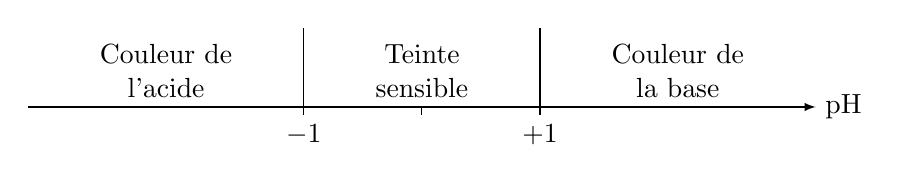
\begin{tikzpicture}
    \draw[-latex] (0,0) -- (10, 0) node[right]{pH}; 
    \draw (3.5, 1) -- ++(0, -1.1) node[below] {$\pKi-1$}; 
    \draw (6.5, 1) -- ++(0, -1.1) node[below] {$\pKi+1$}; 
    \draw (5, 0) -- ++(0, -0.1) node[below] {$\pKi$}; 
    \draw (5,0) node[above, text width=3cm, align=center] {Teinte\\sensible};
    \draw (1.75,0) node[above, text width=3cm, align=center] {Couleur de\\l'acide};
    \draw (8.25,0) node[above, text width=3cm, align=center] {Couleur de\\la base};
  \end{tikzpicture}
\end{center}

Il faudra donc choisir un indicateur coloré de $\pKa$ le proche possible du $\pH$ à l'équivalence, ou au moins que la zone de virage de l'indicateur coloré soit comprise dans le saut de $\pH$ à l'équivalence. De plus, le changement de teinte (zone de virage) se fait à peu près sur deux unités pH (entre $\pKi-1$ et $\pKi+1$. Il faut donc que le saut de pH soit au moins de deux unités pH et qu'il soit très marqué (sinon le virage s'étale sur un grand intervalle de volume).

Dans le tableau ci-dessous, on donne les zones de virage et les couleurs de quelques indicateurs colorés :
\begin{center}
  \begin{tabular}{llll}
\toprule
 Nom  & $\pKi$  & Zone de virage & Couleur acide/base  \\
 \midrule
 Bleu de thymol & \num{2.0} & \num{1.2}-\num{2.8} & rouge/jaune \\
 Hélianthine  & \num{3.7} & \num{3.1}-\num{4.4} &  rouge/jaune  \\
 Rouge de méthyle  & \num{5.2} & \num{4.2}-\num{6.2} &  rouge/jaune  \\
 Bleu de bromothymol  & \num{6.8} & \num{6.0}-\num{7.6} &  jaune/bleu  \\
 Rouge de Crésol  & \num{8.0} & \num{7.2}-{8.8} &  jaune/rouge  \\
 Phénolphtaléine  & \num{9.0} & \num{8.0}-\num{9.9} &  incolore/rouge  \\
 Jaune d'alizarine  & \num{11.0} & \num{10.1}-\num{11.1} &  jaune/violet  \\
 \bottomrule
  \end{tabular}
\end{center}

\section{Manipulations}%
\label{sec:manipulations}

\subsection{Objectif}%
\label{sub:objectif}

L'objectif est de doser l'acide éthanoïque $(\pKa=\num{4.8})$ dans du vinaigre blanc commercial, de façon à déterminer son degré d'acidité, c'est-à-dire la concentration massique en acide éthanoïque dans le vinaigre.

Les résultats obtenus seront comparés et commentés, en tenant compte des informations ci-dessous, tirées de Wikipedia.

\begin{mdframed}
Le vinaigre commun comporte une concentration d'environ 5 à \SI{8}{\percent} en masse d'acide acétique, encore nommé acide éthanoïque, avec des faibles concentrations ou des traces non négligeables d'acide tartrique et d'acide citrique typiques des vinaigres naturels. Les concentrations minoritaires d'autres sels ou solutés chimiques, à l'origine en particulier de saveurs ou goût complémentaires, dépendent de la nature de la solution alcoolique initiale transformée par des enzymes. Ce produit commercial acide, nullement uniformisé malgré l'existence d'une production industrielle parfois massive, est utilisé en particulier dans l'alimentation humaine, notamment dans les préparations culinaires de légumes ou pour la conservation des denrées. Le vinaigre blanc ou vinaigre d'alcool, parfois vendu séché en cristaux est un nettoyant et détachant aujourd'hui considéré comme écologique.
\end{mdframed}

\subsection{Travail préliminaire}%
\label{sub:travail_preliminaire}

La solution titrante est une solution de soude à \SI{0.10}{\mol\per\litre} et le volume de la burette est de \SI{50}{\ml}. Lorsqu'on réalise un titrage, on souhaite que l'équivalence intervienne pour un volume compris entre la moitié et les 2/3 de la burette.

\begin{itemize}
  \item Estimer le volume de vinaigre à prélever pour ce dosage. Commenter. 
  \item Comment améliorer le résultat précédent ?
  \item Quel indicateur coloré doit être utilisé ?
\end{itemize}

\subsection{Titrage}%
\label{sub:titrage}
Réaliser le titrage. On effectuera les trois mesures simultanément en plongeant les électrodes pH-métriques et conductimétriques dans la solution en y ajoutant aussi quelques gouttes d'indicateur coloré.

Déterminer la concentration en acide acétique du vinaigre par les trois méthodes. Le résultat obtenu est-il en accord avec ce qu'on attend du vinaigre ? Comparer la précision des différentes méthodes. 
\end{document}

